\let\textcircled=\pgftextcircled
\chapter{Evaluation}
\label{chap:7}
%----------------------------------------------------------------------------------------
%   INTRO
%----------------------------------------------------------------------------------------
\initial{T}his chapter will draw a parallel line between the initial objectives of the project and the accomplished work. As well as it will cover essential observations during this research. It will assess the accomplished work and do some testing.

\section{Extent of completeness}
\label{subsec:objectives}
As it was mentioned in the introduction chapter the entire project was initially outlined to the 3 main objectives, where each of them has two subsections. 

\subsection{Primary Objectives}
\label{subsec:primary_obj}
\begin{enumerate}[(a)]
    \item The implementation for the generic solver of any level of Nonogram was modelled in \texttt{Essence'} constraint programming language, which is using the tools of Constraint Satisfaction Problems called \texttt{Savile Row} and \texttt{Minion}. The instances of the model is provided by text files, and in the Essence' language all instance files will be having a \texttt{.param} extension. 
    The solver can solve all valid instances, which has at least one valid solution. The instances with one solution will be solved and those instances which has many solutions will also be solved by the Essence' model. The  invalid instances will not have a solution. However, it is not necessarily that it is needed to deal with the instances which has too many solutions. During the implementation it was noticed that some of the instances were having tremendous amount of solutions and could crash the entire computer. Another instances that have big sizes and very complicated distribution of coloured cells, might take too long to be solved. In those cases the problem is still solvable and has one solution but just probably taking too long to be solved. That cases were solved with the help of Minion's preprocessing, which was called \texttt{SACBounds} (shown in Figure \ref{fig:humananddog}). 

    \begin{figure}[tb]
    	\centering
    	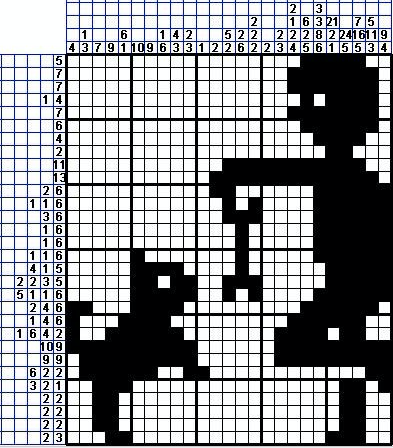
\includegraphics[]{inst_hum}
    	\caption{Hard case instance: "Human and dog" it involves \texttt{SACBounds} tag of Minion}
    	\label{fig:humananddog}
    \end{figure}


    \item Based on this solver it was possible to implement a system which produces all possible valid instances. These instances are tested with the Savile Row and based on that answers it was possible to check whether the instance has one solution or does not. 
\end{enumerate}

\subsection{Secondary Objectives}
\label{subsec:completeness_obj}
\begin{enumerate}[(a)]
    \item To accomplish this objective the valid instance was executed by the Savile Row. Based on the produced solution file(s) it was possible to implement the algorithm which tries to minimise the number of solutions of those instances, which has more than one solution. To get the one solution instance we implemented 2 algorithms: (1) checking only 2 first solutions and based on those pixels which are different in these two solutions decides which pixels should be add and might help in reduction of the solutions; (2) another algorithm takes all solutions, where the amount is less than 10 and based on all the differences between all of them has more iterations, consequently more chances to get one solution instance. To compare these algorithms it was decided to run 100 iterations through both of them and collect the data to the .csv file and do the analysis on R. The testing was made in the following way with the results:
    \begin{verbatim}
	# calculates how many instances did not have a solution
nrow(filtered_data[filtered_data$SolverSolutionsFound == 0,])/2

# removes instances without solutions
filtered_data <- filtered_data[filtered_data$SolverSolutionsFound != 0,]

# separates data by algorithm used
alg1<-subset(filtered_data, filtered_data$UUID==filtered_data$UUID[1])
alg2<-subset(filtered_data, filtered_data$UUID==filtered_data$UUID[nrow(filtered_data)])

# shows how many times each algorithm had to run before all solutions for solvable instances have been found.
nrow(alg1)
# [1] 126
nrow(alg2)
# [1] 169

# splits data by instances
alg1 <- split(alg1, alg1$Filenames)
alg2 <- split(alg2, alg2$Filenames)

# finds the mean number of iteration on an instance each algorithm required to finish
mean(unlist(lapply(alg1, function(x) length(x$SolverSolutionsFound))))
# [1] 1.26
mean(unlist(lapply(alg2, function(x) length(x$SolverSolutionsFound))))
# [1] 1.69

# amount of instances that each algorithm was not able to solve 
length(Filter(function(x) min(x$SolverSolutionsFound) != 1, alg1))
# [1] 39
length(Filter(function(x) min(x$SolverSolutionsFound) != 1, alg2))
# [1] 30
\end{verbatim}

It can be concluded that the algorithms which compares only 2 solution is faster but produces less instances with one solutions than the second algorithm which checks all possible solutions (<10).
    \item After checking that the instance has only one solution it was decided to implement a function which displays the instance in the classic representation. The user can save an print it on the paper later and play it. That is how the instances were printed for the participants of the user study. As well as the user of the system was allowed to decide which parameters is important to be inserted (see Figure \ref{fig:display} )
   \begin{figure}[h]
   	\centering
   	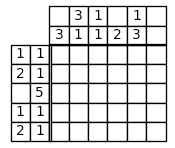
\includegraphics[]{display_inst}
   	\caption{One solution instance that is generated by the system and displayed}
   	\label{fig:display}
   \end{figure}
    
\end{enumerate}


\subsection{Tertiary Objectives}
\label{subsec:tertiary_obj}
\begin{enumerate}[(a)]
    \item Based on the big amount of testing it became more and more apparent with possible properties of the game that could be used to implement the algorithm that will make the level of the instance harder to solve.

    \item However it is not necessarily that computer and human uses the same logic to solve it. Therefore, they might rate the level of the Nonogram differently. This hypothesis was checked by the user study. This part was considered in more details in the User Study chapters.
\end{enumerate}

%----------------------------------------------------------------------------------------
%  SECTION : CONSTRAINT PROGRAMMING
%----------------------------------------------------------------------------------------
\section{Conclusion}
The final section of the entire project will draw the last line about the project in general and about achieved parts. The process of constraint modelling and then development of the the system, which was based on the constraint programming was very engaging. As well as to always discover new logics behind the creation of instances and their enhancement if they could have than more solutions. All the initial objectives of the project were met. Firstly, it was modelling of the constraint satisfaction problem of the Nonogram, then it was the implementation of the different approaches of generating instances and their comparisons, and the last but not the list the implementation of the instance enhancement. The user study was one of the fun part of the research, since it was showing the results of the assumptions made  by the creator of the system. Since the assumptions were made based on logic of the puzzle and computer performance. However, in the future it is possible to conduct more studies involving more participants.

 based on how computer performs the process of  considering some small bit of the human abilities 

 was very engaging and interesting in implementation of the constraint modelling in Essence' as well as involving Python. The most enjoyable part of the project was coding and considere

It was enjoying to do the research in the areas, which involves logic, modelling in constraint programming and at the same time the implementation of the puzzle itself. It was interesting to observe the development of the system that was based on the concept of constraint programming. 


%----------------------------------------------------------------------------------------
%   SUBSECTION:  
%----------------------------------------------------------------------------------------
% \subsection{Subsection}
% \label{subsec:subsec01}

% Begins a subsection.